\documentclass[dvipdfmx,a4paper]{jsarticle}
    \pagestyle{plain}
    \usepackage{amsmath}
    \usepackage{amsthm}
    \usepackage{amssymb}
    \usepackage{graphicx}
    \usepackage{tikz}
    \usepackage{tkz-euclide}
    \usepackage{here}
    \usepackage{cancel}

    \usetikzlibrary{angles}

    \newcommand{\R}{\mathbb{R}}
    \newcommand{\C}{\mathbb{C}}
    \newcommand{\Z}{\mathbb{Z}}
    \newcommand{\N}{\mathbb{N}}
    \newcommand{\Q}{\mathbb{Q}}
    \newcommand{\Lra}{\Leftrightarrow}
    \newcommand{\al}{\alpha}
    \newcommand{\be}{\beta}
    \newcommand{\ga}{\gamma}
    \newcommand{\om}{\omega}
    \newcommand{\De}{\Delta}
    \newcommand{\oraw}{\overrightarrow}
    \newcommand{\bs}{\backslash}
    \newcommand{\2}{I\hspace{-1pt}I}
    \newcommand{\3}{I\hspace{-1pt}I\hspace{-1pt}I}

    \newtheorem{cs}{Case}
    \newtheorem{cas}{Case}
    \newtheorem{case}{Case}
    \newtheorem{apf}{別解}
    \newtheorem{anpf}{別解}

    \usetikzlibrary{calc}
    \title{2022年度京大数学(文系)の解答}
    \author{tt0801}
    \date{\today}
    
    \begin{document}
    \maketitle
    \section{大問1}
    \subsection{問題}
    $5.4 < \log_4 2022 < 5.5$であることを示せ. ただし, $0.301 < \log_{10} 2 < 0.3011$であることは用いてよい. 


    \subsection{解答}
    \begin{align*}
        \log_4 2022 &= \dfrac{\log_{10} 2022}{\log_{10} 4} \\
            &= \dfrac{\log_{10} 2 + \log_{10} 1011}{2\log_{10} 2} \\
            &= \dfrac{1}{2} + \dfrac{\log_{10} 1011}{2\log_{10} 2} \ (=A \mathrm{とおく})
    \end{align*}
    である. ここで, $\log_{10} 1011 > \log_{10} 1000 = 3$より, 
    \begin{align*}
        A & > \dfrac{1}{2} + \dfrac{3}{2\log_{10} 2} \\
        & > \dfrac{1}{2} + \dfrac{3}{2\cdot 0.3011} \ (\because \log_{10} 2 < 0.3011)\\
        &= \dfrac{33011}{6022} \\
        &> 5.4
    \end{align*}
    なので, $\log_4 2022 > 5.4$である. 
    
    また, $\log_{10} 1011 < \log_{10} 1024 = 10 \log_{10} 2$なので, 
    \begin{align*}
        A & < \dfrac{1}{2} + \dfrac{10 \log_{10} 2}{2\log_{10} 2} \\
        &= \dfrac{1}{2} + 5\\
        &= 5.5
    \end{align*}
    である. よって, $\log_4 2022 < 5.5$となる. 

    以上より, $5.4 < \log_4 2022 < 5.5$が示された. 


    \subsection{解説}
    $\log_{10} 2$の評価式が与えられているので, $\log_{10} 2$を作ることを意識して式変形をする. 

    \section{大問2}
    \subsection{問題}
    下図の三角柱$\mathrm{ABC - DEF}$において, Aを始点として, 辺に沿って頂点を$n$回移動する. すなわち, 
    この移動経路
    \begin{equation*}
        \mathrm{
            P_0 \rightarrow P_1 \rightarrow P_2 \rightarrow \cdots 
            \rightarrow P_{n-1} \rightarrow P_n \quad (\mathrm{ただし} P_0 = A)
        }
    \end{equation*}
    において, $\mathrm{P_0P_1, P_1P_2, \cdots, P_{n-1}P_n}$はすべて辺であるとする. また, 
    同じ頂点を何度通ってもよいものとする. このような移動経路で, 終点$\mathrm{P_n}$が
    $\mathrm{A, B, C}$のいずれかとなるものの総数$a_n$を求めよ. 

    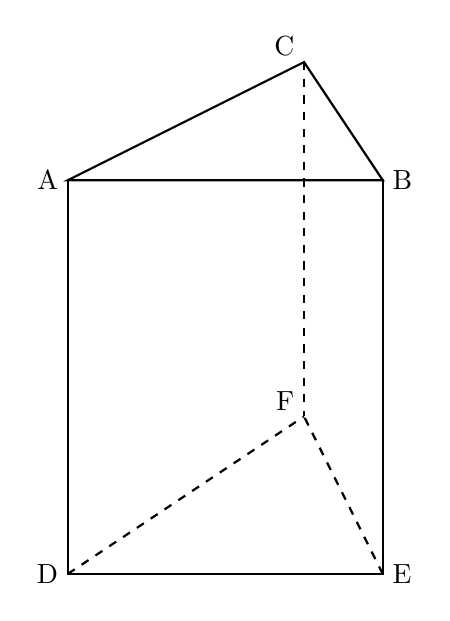
\begin{tikzpicture}
        % Draw the base square A - B - E - D
        \draw[thick] (0,0) -- (4,0) -- (4,-5) -- (0,-5) -- cycle;

        % Draw the top triangle A - C - B
        \draw[thick] (0,0) -- (3,1.5) -- (4,0) -- cycle;

        % Connect base to apex of the triangle C - F
        \draw[thick, dashed] (3,1.5) -- (3,-3);

        % Draw the diagonal lines of the base D - F, E - F
        \draw[thick, dashed] (0,-5) -- (3,-3);
        \draw[thick, dashed] (4,-5) -- (3,-3);

        % Label the points
        \node[anchor=east] at (0,0) {A};
        \node[anchor=west] at (4,0) {B};
        \node[anchor=east] at (3,1.7) {C};
        \node[anchor=east] at (0,-5) {D};
        \node[anchor=west] at (4,-5) {E};
        \node[anchor=east] at (3,-2.8) {F};
    \end{tikzpicture}

    \subsection{解答}
    各頂点から隣接する他の頂点に移動する方法は, 3通りである. よって, $n$回移動した時の全ての経路の
    場合の数は, $3^n$である. $b_n = 3^n-a_n$とおくと, 終点$\mathrm{P_n}$が
    $\mathrm{D,E,F}$のいずれかとなるものの総数である. 

    $\mathrm{P_n}$が頂点$\mathrm{A,B,C}$のいずれかにいる時, 
    $\mathrm{P_{n+1}}$が再び頂点$\mathrm{A,B,C}$のいずれかにいる経路は2通りである. 
    一方で, $\mathrm{P_n}$が頂点$\mathrm{D,E,F}$のいずれかにいる時, 
    $\mathrm{P_{n+1}}$が頂点$\mathrm{A,B,C}$のいずれかにいる経路は1通りである. 
    以上より, 
    \begin{align*}
        a_{n+1} &= 2a_n + b_n \\
                &= 2a_n + (3^n-a_n) \\
                &= a_n + 3^n
    \end{align*}
    を得る. $a_0=1$とおけば, この漸化式は0以上の整数$n$で成立する. 
    $n \geq 1$の場合は, 
    \begin{align*}\displaystyle
        a_n &= a_0 + \sum_{k=0}^{n-1} (a_{k+1} - a_k) \\
            &= 1 + \sum_{k=0}^{n-1} 3^k \\
            &= 1 + \dfrac{3^n-1}{3-1} \\
            &= \dfrac{3^n+1}{2}
    \end{align*}
    が成り立つ. これは, $n=0$の場合も成立. 

    以上より, 
    \begin{equation*}
        a_n = \dfrac{3^n+1}{2}.
    \end{equation*}
    

    \subsection{解説}
    $\mathrm{P_n}$の位置について, 事象は次の2通りしかない. 
    \begin{itemize}
        \item $\mathrm{P_n}$は$\mathrm{A, B, C}$のいずれか, 
        \item $\mathrm{P_n}$は$\mathrm{D, E, F}$のいずれか. 
    \end{itemize}
    図の対称性から, これらの事象について漸化式を立てられそうだと見通しがつく. 


    \section{大問3}
    \subsection{問題}
    $xy$平面上の2直線$L_1, L_2$は直交し, 交点の$x$座標は$\dfrac{3}{2}$である. また, 
    $L_1, L_2$はともに曲線$C: y = \dfrac{x^2}{4}$に接している. 
    このとき, $L_1, L_2$および$C$で囲まれる図形の面積を求めよ. 

    \subsection{解答}
    $f(x) = \dfrac{x^2}{4}$とおく. $f'(x) = \dfrac{x}{2}$である. 
    $L_1$と$C$の接点の座標を$(p, f(p))$, $L_2$と$C$の接点の座標を$(q, f(q))$とおく. 
    $L_1$は$x=p$における$C$の接線であるので, その方程式は$y-f(p) = f'(p)(x-p)$, すなわち, 
    \begin{equation} \label{pb3_eq1}
        y = \dfrac{p}{2} x - \dfrac{p^2}{4}
    \end{equation}
    である. 同様に$L_2$の方程式は, 
    \begin{equation} \label{pb3_eq2}
        y = \dfrac{q}{2} x - \dfrac{q^2}{4}
    \end{equation}
    で与えられる. $L_1, L_2$は直交するので, 傾きの積$\dfrac{p}{2} \cdot \dfrac{q}{2}$
    が$-1$に等しい. よって, 
    \begin{equation} \label{pb3_eq3}
        pq = -4.
    \end{equation}
    特に$p \neq q$である. 
    また, $L_1$と$L_2$の交点の座標は, 方程式(\ref{pb3_eq1}), (\ref{pb3_eq2})を連立して, 
    $\left(\dfrac{p+q}{2}, \dfrac{pq}{4}\right)$と分かる. 
    問題文の条件より$\dfrac{p+q}{2} = \dfrac{3}{2}$, すなわち
    \begin{equation} \label{pb3_eq4}
        p + q = 3
    \end{equation}
    である. 式(\ref{pb3_eq3}),(\ref{pb3_eq4})より, $p,q$は$t$についての二次方程式
    $t^2 -3t -4 = 0$の解である. 因数分解して$(t-4)(t+1)=0$なので, 
    \begin{equation*}
        (p,q) = (-1, 4)
    \end{equation*}
    として一般性を失わない. この時, 
    \begin{align*}
        L_1 :& y =  -\dfrac{1}{2} x - \dfrac{1}{4}, \\
        L_2 :& y =  2 x - 4.
    \end{align*}
    である. 

    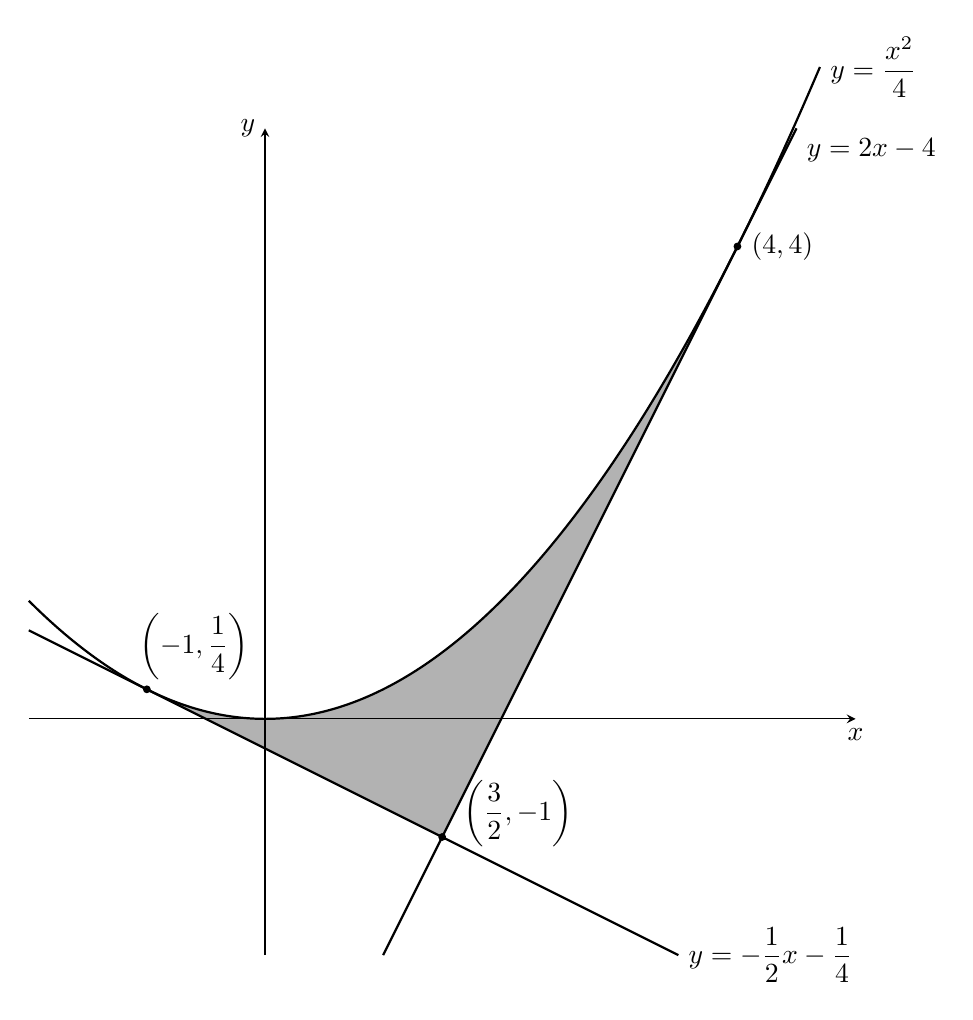
\begin{tikzpicture}[scale=1.5, >=stealth]

        % Draw axes
        \draw[->] (-2,0) -- (5,0) node[below] {$x$};
        \draw[->] (0,-2) -- (0,5) node[left] {$y$};
        
        % Plot y = -1/2 x - 1/4
        \draw[thick, black, domain=-2:3.5] plot(\x, {-0.5*\x - 0.25}) node[right] {$y = -\dfrac{1}{2}x - \dfrac{1}{4}$};
        
        % Plot y = 2x - 4
        \draw[thick, black, domain=1:4.5] plot(\x, {2*\x - 4}) node[below right] {$y = 2x - 4$};
        
        % Plot y = x^2 / 4
        \draw[thick, black, domain=-2:4.7, samples=200] plot(\x, {\x*\x/4}) node[right] {$y = \dfrac{x^2}{4}$};
        
        % Fill the enclosed area
        \begin{scope}
            \clip (-2,-2) rectangle (5,5); % Restrict to visible region
            \fill[black, opacity=0.3] 
            plot[domain=-1:4, samples=200] (\x, {\x*\x/4}) --
                plot[domain=4:1.5, samples=200] (\x, {2*\x - 4}) -- % Line y = 2x - 4
                plot[domain=1.5:-1, samples=200] (\x, {-0.5*\x - 0.25}) -- cycle;% Line y = -1/2x - 1/4
        \end{scope}
        
        % Add intersection points as labels
        \node[circle, fill=black, inner sep=1pt] at (-1, 0.25) {};
        \node[above] at (-0.6,0.25) {$\left(-1, \dfrac{1}{4}\right)$};
        \node[circle, fill=black, inner sep=1pt] at (1.5, -1) {};
        \node[right] at (1.6,-0.8) {$\left(\dfrac{3}{2}, -1\right)$};
        \node[circle, fill=black, inner sep=1pt, label=right:{$(4, 4)$}] at (4, 4) {};
        
        
    \end{tikzpicture}

    求める面積$S$は上図の色塗られた領域の面積であるから, 
    \begin{align*}\displaystyle
        S &= \int_{-1}^{\frac{3}{2}} \frac{x^2}{4} - \left(-\frac{1}{2}x -\frac{1}{4}\right) \ dx 
        + \int_{\frac{3}{2}}^{4} \frac{x^2}{4} - \left(2x -4\right) \ dx \\
        &= \int_{-1}^{\frac{3}{2}} \frac{1}{4}\left(x + 1\right)^2 \ dx 
        + \int_{\frac{3}{2}}^{4} \frac{1}{4}\left(x -4\right)^2 \ dx \\
        &= \left[ \frac{1}{12}(x+1)^3\right]_{-1}^{\frac{3}{2}}
        + \left[ \frac{1}{12}(x-4)^3\right]_{\frac{3}{2}}^{4} \\
        &= \frac{1}{12} \left(\frac{5}{2}\right)^3
        - \frac{1}{12} \left(-\frac{5}{2}\right)^3 \\
        &= \frac{125}{48}
    \end{align*}
    と求まる. 

    以上より, 求める面積は$\dfrac{125}{48}$である. 

    \subsection{解説}
    覚える必要は全くないが, 問題の面積は, いわゆる$\dfrac{1}{6}$公式で求まる面積の半分なので, 
    知っていれば検算は容易である. 

\end{document}